\subsection{The $\pi$-calculus}
\label{sec:PA}

\subsubsection{Syntax and Notations}

The $\pi$-calculus \cite{pi_paper, pi_book} is a name passing calculus, in the sense that computations are represented by passing $\it{names}$ through $\it{channels}$.  The $\pi$-calculus uses lower-case letter to denote a name, which could be either a channel or a variable.  

Syntax of the $\pi$-calculus given in Table \ref{pi-syn} also denotes part of its semantics.  The prefix of a process denotes its capability, which could be  
\begin{inparaenum}[(i)]
  \item receiving names from a channel;
  \item sending names through a channel; or
  \item performing an internal action that cannot be observed from outside.
\end{inparaenum}
Informally, a process could :
\begin{inparaenum}[(1)]
  \item evolve to another process after performing an action;
  \item evolve as two processes who are running at the same time;
  \item evolve as one of the two processes;
  \item evolve to another process when two names become equal;
  \item a process with a private name;
  \item infinite parallel composition of the same process; or
  \item an inert process that does nothing.
\end{inparaenum}
Finally, two processes are structurally congruent, $\equiv$, if they are equal up to structure rules listed in Table \ref{pi-str-cong}

In the rest of this section, we distinguish reduction relation($\longrightarrow$) from labelled transition relations($\overset{\alpha}{\longrightarrow}$).  Specifically, the assertion $P \longrightarrow P'$ states that process $P$ can evolve to process $P'$ as a result of an action {\it{within}} $P$.  On the other hand, $P \overset{\alpha}{\longrightarrow} Q$ indicates that $P$ can evolve to Q after performing action $\alpha$.  Reduction relations are formally defined in Table \ref{pi-str-red} and transition relations are formally defined in Table \ref{pi-trans}.

\begin{table}[h]
  \begin{center}
  \begin{tabular}{ l c l  l l c l  l }
$\alpha$&:: = &                                                                    	& action           &P & :: =  & & process \\
              & $|$ & $u(\widetilde{x}$)                                       	& input            &   & $|$  & $ \alpha.P$&prefix\\
              & $|$ & $\overline{u} \langle \widetilde{y} \rangle$	& output          &   & $|$ &$P\ |\ P$& composition\\
              & $|$ & $\tau$                                                         	& silent/internal & & $|$ &$P\ +\ P$& summation\\
                                                                                                                 &&&&& $|$ &$ [x = y].P $& match \\
                                                                                                                 &&&&& $|$ & $(\mathit{\nu}x).P$&restriction\\
                                                                                                                 &&&&& $|$ & $!P$ & replication\\
                                                                                                                 &&&&& $|$ & 0 & inert process\\                                                                                                                 
  \end{tabular}
  \end{center}
  \caption{Syntax of the $\pi$-calculus}
  \label{pi-syn}
\end{table}

\begin{table}[h]
  \begin{center}
  \begin{tabular}{ l r c l }
  SC-MAT					&$[x = x] \alpha.P$			&$\equiv$&$\alpha.P$\\
  SC-SUM-ASSOC		&$P_1\ +\ (P_2\ +\ P_3)$	&$\equiv$&$(P_1\ +\ P_2)\ +\ P_3$\\
  SC-SUM-COMM		&$P_1\ +\ P_2$				&$\equiv$&$P_2\ +\ P_1$\\
  SC-SUM-INACT		&$P\ +\ 0$					&$\equiv$&$P$\\
  SC-COMP-ASSOC	&$P_1\ |\ (P_2\ |\ P_3)$	&$\equiv$&$(P_1\ |\ P_2)\ |\ P_3$\\
  SC-COMP-COMM		&$P_1\ |\ P_2$				&$\equiv$&$P_1\ |\ P_2$\\
  SC-COMP-INACT		&$P\ |\ 0$						&$\equiv$&$P$\\
  SC-RES					&$\nu z\ \nu w\ P$			&$\equiv$&$\nu w\ \nu z\ P$\\
  SC-RES-INACT		&$\nu z\ 0$					&$\equiv$&$0$\\
  SC-RES-COMP		&$\nu z\ (P_1\ |\ P_2)$		&$\equiv$&$P_1\ |\  \nu z\ P_2, if\ z\not{\in} fn(P_1)$\\
  SC-REP					&$!P$							&$\equiv$&$P\ |\ !P$\\
  \end{tabular}
  \end{center}
  \caption{The axioms of structural congruence}
  \label{pi-str-cong}
\end{table}

\vspace{20 mm}

\begin{table} [H]
  \begin{center}

  \begin{tabular}{ c c }
\multicolumn{2}{c}{R-INTER $\frac{}{(\bar{x}\langle y \rangle.P_1\ +\ M_1)\ |\ (x(z).P_2\ +\ M_2)\ \longrightarrow\ P_1\ |\ P_2\{y/z\}}$}\\
\\
R-PAR $\frac{P_1\ \longrightarrow\ P^{'}_{1}}{P_1\ |\ P_2\ \longrightarrow\ P^{'}_{1}\ |\ \ P_{2}}$ & 
R-RES $\frac {P\ \longrightarrow\ P^{'}} {\nu z P\ \longrightarrow\ \nu z P^{'}} $\\
\\
R-STRUCT $\frac {P_1\ \equiv\ P_2\ \ P_2\ \longrightarrow\ P_2^{'}\ \ P_2^{'}\ \equiv\ P_1^{'}\ } {P_1\ \longrightarrow\ P^{'}_{1}} $&
R-TAU $\frac {} {\tau  P\ + \ M\ \longrightarrow\ P}$
  \end{tabular}
  \end{center}
  \caption{Reduction rules in the $\pi$-calculus}
  \label{pi-str-red}
\end{table}

\vspace{10 mm}

\begin{table}[H]
  \begin{center}
  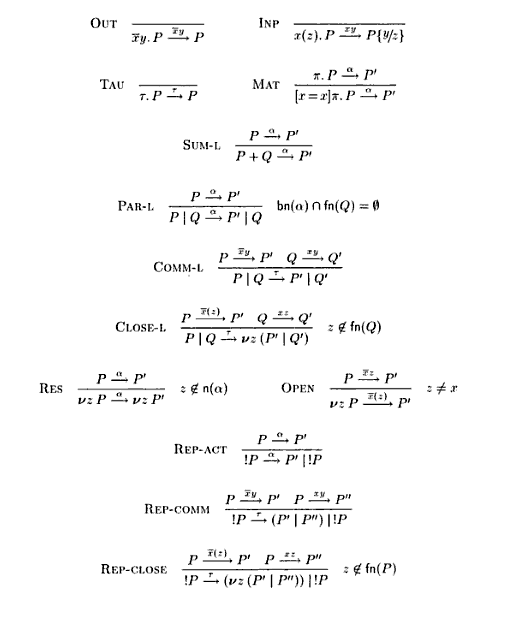
\includegraphics[scale=0.4]{pi_trans.png}
  \end{center}
  \caption{Transition rules in the $\pi$-calculus}
  \label{pi-trans}
\end{table}


\subsubsection{Equivalence Relations}

Equivalence relations are important concepts in an algebraic system.  Unfortunately, the variety of equivalence relations in the $\pi$-calculus and other classical process calculi are usually obstacles to learning a calculus.  This section will give a gentle introduction to the most important equivalence relation in the $\pi$-calculus, the strong barbed bisimulation, followed by short definitions cited from \cite{pi_book} in a designed order.  By reading this section, readers will obtain a basic understanding for all equivalences in the Figure \ref{pi-eq} and most other common equivalences in literature.


$\bf{Barbed\ relations}$ study the behaviour of a process via examining its potential interactions with the environment.  Formally,

\begin{defn}
For each name or co-name $\mu$, the observability predicate $\downarrow_\mu$ is defined by:\\
    (1) P $\downarrow_\mu$ if P can perform an input action via channel $\mu$\\
    (2) P $\downarrow_\text{$\overline{\mu}$}$ if P can perform an output action via channel $\mu$
\end{defn}
 
Strong barbed relations can be defined as follows:

\begin{defn}
A relation S is a $\mathbf{strong\ barbed\ bisimulation}$ if whenever (P,Q) $\in$ S,\\
(1) P $\downarrow_\mu$ implies Q$\downarrow_\mu$\\
(2) P $\overset{\tau}{\longrightarrow}$ P' implies Q $\overset{\tau}{\longrightarrow}$ Q' for some Q' with (P', Q') $\in$ S \\
(3) Q $\downarrow_\mu$ implies P$\downarrow_\mu$\\
(4) Q $\overset{\tau}{\longrightarrow}$ Q' implies P $\overset{\tau}{\longrightarrow}$ P' for some P' with (P', Q') $\in$ S
\end{defn}

\begin{defn}
P and Q are $\mathbf{strong\ barbed\ bisimilar}$ if (P,Q) $\in$ S for some barbed bisimulation S.
\end{defn}

\begin{defn}
P and Q are $\mathbf{strong\ barbed\ congruence}$ if C[P] and C[Q] are strong barbed bisimilar for any context C\footnote{A context, $C[\cdot]$ is a term written using the same syntax of the $\pi$-calculus and an additional constant $\cdot$.  Substituting the $\cdot$ by a process P result in a $\pi$-calculus term $C[P]$ }.
\end{defn}

\begin{defn}
P and Q are $\mathbf{strong\ barbed\ equivalent}$ if P $|$ R and Q $|$ R are strong barbed bisimilar for any process R.
\end{defn}

$\bf{Bisimulation,\ bisimilarity,\ congruence,\ and\ equivalent}$, as revealed in the barbed relations, are four related concepts in process calculi.  For this reason, in the rest of this subsection, where various of equivalent relations will be introduced, only one of the four concepts in each group will be defined explicitly.  The meaning of the rest three relations in each group should be apparent. 

\begin{defn}
A relation S is a $\mathbf{reduction\ bisimulation}$ if whenever (P,Q) $\in$ S,\\
(1) P $\overset{\tau}{\longrightarrow}$ P' implies Q $\overset{\tau}{\longrightarrow}$ Q' for some Q' with (P', Q') $\in$ S \\
(2) Q $\overset{\tau}{\longrightarrow}$ Q' implies P $\overset{\tau}{\longrightarrow}$ P' for some P' with (P', Q') $\in$ S
\end{defn}

In terms of evaluation strategy, the $\pi$-calculus could adopt either the early instantiation scheme or the late instantiation scheme.  In the early instantiation scheme, variables are instantiated as soon as an input message is received, more precisely, $\frac{-}{a(x).P\ \overset{av}{\longrightarrow}P\{v/x\}}$.  On the contrary, in the late instantiation scheme, bound variables of input actions are instantiated only when they are involved in an internal communication.

\begin{defn}
A binary relation S on processes $P$ and $Q$ is an $\mathbf{early\ simulation}$, $\sim_e$,  if PSQ implies that\\
1. If P $\overset{\alpha}{\longrightarrow}$ P' and $\alpha$ is a free action\footnote{an internal action or a free output.}, then for some Q', Q $\overset{\alpha}{\longrightarrow}$ Q' and P'SQ'\\
2. If P $\overset{x(y)}{\longrightarrow}$ P' and y$\not{\in}$ n(P,Q), then for all w, there is Q' such that Q$\overset{x(y)}{\longrightarrow}$ Q' and P\{w/y\}SQ\{w/y\}\\
3. If P $\overset{\bar{x}(y)}{\longrightarrow}$ P' and y$\not{\in}$ n(P,Q), then for some Q', Q $\overset{\bar{x}(y)}{\longrightarrow}$ Q' and P'SQ'
\end{defn}

\begin{defn}
A binary relation S on agents is a $\mathbf{late \ simulation}$, $\sim_l$,  if PSQ implies that\\
1. If P $\overset{\alpha}{\longrightarrow}$ P' and $\alpha$ is a free action, then for some Q', Q $\overset{\alpha}{\longrightarrow}$ Q' and P'SQ'\\
2. If P $\overset{x(y)}{\longrightarrow}$ P' and y$\not{\in}$ n(P,Q), then for some Q', Q$\overset{x(y)}{\longrightarrow}$ Q' and for all w, P\{w/y\}SQ\{w/y\}\\
3. If P $\overset{\bar{x}(y)}{\longrightarrow}$ P' and y$\not{\in}$ n(P,Q), then for some Q', Q $\overset{\bar{x}(y)}{\longrightarrow}$ Q' and P'SQ'
\end{defn}

\begin{defn}
P and Q are $\mathbf{full\ bisimilar}$, P $\approx^c$ Q	, if P$\sigma\ \approx$ Q$\sigma$ for every substitution $\sigma$.
\end{defn}

\begin{defn}
A binary relation R over processes is an $\mathbf{open\ bisimulation}$, $\approx_o$, if for every pair of elements (p,q) $\in$ R and for every name substitution $\sigma$ and every action $\alpha$, whenever p$\sigma \overset{\alpha}{\longrightarrow}$ p' then there exists some q' such that q$\sigma\overset{\alpha}{\longrightarrow}$q' and (p', q') $\in$ R.
\end{defn}

\begin{defn}
A relation is $\mathbf{ground\ bisimulation}$, $\approx_g$, iff whenever P $\approx_g$ Q, there is z$\not{\in}$fn(P, Q) such that if P$\overset{\alpha}{\longrightarrow}$Q, where $\alpha$ is an action, then then Q$\overset{\alpha}{\Rightarrow }\approx_g$P.
\end{defn}

To conclude this subsection, Figure \ref{pi-eq}, cited from \cite{pi_book}, presents the hierarchy of equivalences in the $\pi$-calculus.

\begin{figure} [h]
  \begin{center}

\begin{picture}(100, 160)
  \put(90, 160){$weakest$}
  \put(100, 80){\vector(0,1){70}}
  \put(100, 80){\vector(0,-1){70}}
  \put(90, 0){$strongest$}
  
  \put(50,160){$\approx_g$}
  \put(60,130){\line(0,1){20}}
  \put(50,120){$\approx,\ \cong$}
  \put(45,90){\line(2,3){14}}
  \put(60,90){\line(0,1){20}}
  \put(0,80){$\approx_g^c,\ \approx^c,\ \cong^c$}
  \put(60,80){$\approx_l$}
  \put(45,55){\line(2,3){14}}
  \put(45,55){\line(0,1){20}}
  \put(45,40){$\approx_l^c$}
  \put(45,15){\line(0,1){20}}
  \put(45,0){$\approx_o$}
\end{picture}
  \end{center}

  \begin{center}
  \begin{tabular}{ c l c l c l}
$\approx_g:$&$ground\ bisimilarity$&$\approx:$&$bisimilarity$&$\cong:$&$barbed\ equivalence$\\
$\approx_g^c:$&$ground\ congruence$&$\approx^c:$&$full\ bisimilarity$&$\cong^c:$&$barbed\ congruence$\\
$\approx_l:$&$late\ bisimilarity$&$\approx_l^c:$&$late\ congruence$&$\approx_o:$&$open\ bisimilarity$\\
  \end{tabular}
  \end{center}
  \caption{Hierarchy of equivalences in the $\pi$-calculus}
  \label{pi-eq}
\end{figure}

